\providecommand{\main}{../../..}
\documentclass[\main/main.tex]{subfiles}
\begin{document}

\subsection{Esercizio 2}
Dato il problema di programmazione matematica

\begin{align*}
  \min f(x) & =x^2_1+x^2_2           \\
  g_1(x)    & = 1-x_1x_2 \leq 0      \\
  g_2(x)    & = x_1 + x_2 -4 \leq 0  \\
  g_3(x)    & = -x_1 - x_2 - 2\leq 0
\end{align*}

\begin{enumerate}[a)]
  \item Si rappresenti il problema graficamente.
  \item Si determinino gli eventuali punti non regolari o si mostri che non ne esistono.
  \item Si determinino i punti candidati secondo le condizioni di KKT, e in particolare quello/i di minimo.
\end{enumerate}

\subsection{Soluzione esercizio 2}

\paragraph*{a) La funzione nel suo dominio di definizione è la seguente:}

\begin{figure}
  \begin{subfigure}{0.45\textwidth}
    \xygraph{0}{4}{0}{4}{0}{1-x*y < 0 && x + y < 4 && -x - y < 2}{y^2+x^2}
    \caption{La funzione $f(x)$}
  \end{subfigure}
  ~
  \begin{subfigure}{0.45\textwidth}
    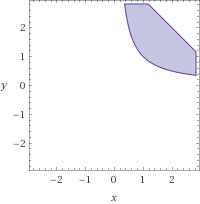
\includegraphics[width=0.8\textwidth]{11042016domain}
    \caption{Dominio della funzione $f(x)$}
  \end{subfigure}
  \caption{La funzione nella regione ammissibile}
\end{figure}

\paragraph*{Calcolo dei punti non regolari:}
Calcolo i gradienti dei vincoli:
\[
  \nabla g_1 = \begin{bmatrix}
    -x_2 \\
    -x_1
  \end{bmatrix}
  \qquad
  \nabla g_2 = \begin{bmatrix}
    1 \\
    1
  \end{bmatrix}
  \qquad
  \nabla g_3 = \begin{bmatrix}
    -1 \\
    -1
  \end{bmatrix}
\]

Il gradiente $ \nabla g_1$ si annulla nell'origine, che è all'esterno del dominio di interesse (nessun vincolo è attivo in quel punto). Gli altri gradienti $ \nabla g_2$ e $\nabla g_3$ non si annullano.

Calcolo i punti dati dall'intersezione dei vincoli a coppie:

\subparagraph*{Vincoli $g_1$ e $g_2$:}

\[
  \begin{cases}
    1-x_1x_2 = 0 \\
    x_1 + x_2 - 4 = 0
  \end{cases}
  \Rightarrow
  \begin{cases}
    1-x_2(4 - x_2) = 0 \\
    x_1  = 4 - x_2
  \end{cases}
  \Rightarrow
  \begin{cases}
    x^2_2 - 4x_2 +1 = 0 \Rightarrow x_2 = 2 \pm \sqrt{3} \\
    x_1  = 4 - x_2
  \end{cases}
\]

Da cui deriviamo i punti $A = (2 + \sqrt{3}, 2 - \sqrt{3})$ e $B = (2 - \sqrt{3}, 2 + \sqrt{3})$. In nessuno di questi punti la matrice realizzata accostando i gradienti risulta singolare, quindi i punti $A$ e $B$ sono regolari.

\subparagraph*{Vincoli $g_1$ e $g_3$:}

\[
  \begin{cases}
    1-x_1x_2 = 0 \\
    x_1  = -x_2 - 2
  \end{cases}
  \Rightarrow
  \begin{cases}
    1+(x_2 + 2)x_2 = 0 \\
    x_1  = -x_2 - 2
  \end{cases}
  \Rightarrow
  \begin{cases}
    1+x^2_2 +2x_2 = 0 \Rightarrow x_2 = -1 \\
    x_1  = -1
  \end{cases}
\]

Ne deriviamo il punto $C = (-1, -1)$ che viene identificato come punto non regolare ed è quindi aggiunto alla lista dei punti candidati.

\subparagraph*{Vincoli $g_2$ e $g_3$:}
I due vincoli non hanno intersezioni.

\subparagraph*{Vincoli $g_1$, $g_2$ e $g_3$:}
I tre vincoli non hanno intersezioni comuni.

\paragraph*{Condizioni KKT}
\subparagraph*{Realizzo il sistema delle condizioni KKT}

\[
  \begin{cases}
    \begin{bmatrix}
      2x_1 \\
      2x_2
    \end{bmatrix} -
    \mu_1 \begin{bmatrix}
      x_2 \\
      x_1
    \end{bmatrix} +
    \mu_2 \begin{bmatrix}
      1 \\
      1
    \end{bmatrix} -
    \mu_3 \begin{bmatrix}
      1 \\
      1
    \end{bmatrix} = \bm{0} \\
    \mu_1 (1-x_1x_2) = 0                      \\
    \mu_2 (x_1 + x_2 -4) = 0                  \\
    \mu_3 (-x_1 - x_2 - 2) = 0                \\
    1-x_1x_2 \leq 0                           \\
    x_1 + x_2 -4 \leq 0                       \\
    -x_1 - x_2 - 2 \leq 0                     \\
    \mu_1 \geq 0                              \\
    \mu_2 \geq 0                              \\
    \mu_3 \geq 0                              \\
  \end{cases}
  \Rightarrow
  \begin{cases}
    2x_1-\mu_1x_2 + \mu_2 - \mu_3 = 0 \\
    2x_2-\mu_1x_1 + \mu_2 - \mu_3 = 0 \\
    \mu_1 (1-x_1x_2) = 0              \\
    \mu_2 (x_1 + x_2 -4) = 0          \\
    \mu_3 (-x_1 - x_2 - 2) = 0        \\
    1-x_1x_2 \leq 0                   \\
    x_1 + x_2 -4 \leq 0               \\
    -x_1 - x_2 - 2 \leq 0             \\
    \mu_1 \geq 0                      \\
    \mu_2 \geq 0                      \\
    \mu_3 \geq 0                      \\
  \end{cases}
\]
Iniziamo l'albero di ricerca da $\mu_1$:

\begin{figure}
  \begin{tikzpicture}
    \Tree[.$root$
      [.$\mu_1=0$ ]
        [.$\mu_1>0$ ]
    ]
  \end{tikzpicture}
  \caption{Albero di ricerca, primo step}
\end{figure}

Inizio dal caso $\mu_1=0$:

\[
  \begin{cases}
    2x_1 + \mu_2 - \mu_3 = 0   \\
    2x_2 + \mu_2 - \mu_3 = 0   \\
    \mu_2 (x_1 + x_2 -4) = 0   \\
    \mu_3 (-x_1 - x_2 - 2) = 0 \\
    1-x_1x_2 \leq 0            \\
    x_1 + x_2 -4 \leq 0        \\
    -x_1 - x_2 - 2 \leq 0      \\
    \mu_1 = 0                  \\
    \mu_2 \geq 0               \\
    \mu_3 \geq 0               \\
  \end{cases}
  \Rightarrow
  \begin{cases}
    x_1 = x_2                   \\
    \mu_2 (2x_1 -4) = 0         \\
    \mu_3 (-2x_1 - 2) = 0       \\
    x_1 \geq 1 \lor x_1 \leq -1 \\
    x_1 \leq 2                  \\
    x_1 \geq -1                 \\
    \mu_1 = 0                   \\
    \mu_2 \geq 0                \\
    \mu_3 \geq 0                \\
  \end{cases}
  \Rightarrow
  \begin{cases}
    x_1 = x_2            \\
    \mu_2 (2x_1 -4) = 0  \\
    \mu_3 (2x_1 + 2) = 0 \\
    1 \leq x_1 \leq 2    \\
    \mu_1 = 0            \\
    \mu_2 \geq 0         \\
    \mu_3 \geq 0         \\
  \end{cases}
\]
Noto che, se $x_1$ e $x_2$ sono vincolati tra $1$ e $2$, allora la relazione $\mu_3 (2x_1 + 2) = 0$ implica che $\mu_3=0$:

\[
  \begin{cases}
    x_1 = x_2           \\
    \mu_2 (2x_1 -4) = 0 \\
    1 \leq x_1 \leq 2   \\
    \mu_1 = 0           \\
    \mu_2 \geq 0        \\
    \mu_3 = 0           \\
  \end{cases}
  \Rightarrow
  \begin{cases}
    x_1 = x_2           \\
    \mu_2 = -2x_1       \\
    -2x_1 (2x_1 -4) = 0 \\
    1 \leq x_1 \leq 2   \\
    \mu_1 = 0           \\
    \mu_2 \geq 0        \\
    \mu_3 = 0           \\
  \end{cases}
  \Rightarrow
  \error{\mu_2 = -4 < 0}
\]
Ora, $x_1 \neq 0$, per cui $x_1 = 2$. Ma questo implica che $\mu_2 = -4 < 0$, per cui questa opzione risulta impossibile.

Esploriamo, nel ramo $\mu_1 > 0$ l'opzione $\mu_2$.

\begin{figure}
  \begin{tikzpicture}
    \Tree[.$root$
      [.$\mu_1=0$
          [.\error{$\mu_2 = -4 < 0$} ]
        ]
        [.$\mu_1>0$
          [.$\mu_2=0$ ]
            [.$\mu_2>0$ ]
        ]
    ]
  \end{tikzpicture}
  \caption{Albero di ricerca, secondo step}
\end{figure}

Inizio dall'opzione $\mu_2=0$:

\[
  \begin{cases}
    2x_1-\mu_1x_2  - \mu_3 = 0 \\
    2x_2-\mu_1x_1  - \mu_3 = 0 \\
    x_1x_2 = 1                 \\
    \mu_3 (-x_1 - x_2 - 2) = 0 \\
    x_1 + x_2 -4 \leq 0        \\
    -x_1 - x_2 - 2 \leq 0      \\
    \mu_1 > 0                  \\
    \mu_2 = 0                  \\
    \mu_3 \geq 0               \\
  \end{cases}
\]
Esploro ulteriormente le opzioni $\mu_3$ come sottorami:


\begin{figure}
  \begin{tikzpicture}
    \Tree[.$root$
      [.$\mu_1=0$
          [.\error{$\mu_2 = -4 < 0$} ]
        ]
        [.$\mu_1>0$
          [.$\mu_2=0$
              [.$\mu_3=0$ ]
                [.$\mu_3>0$ ]
            ]
            [.$\mu_2>0$ ]
        ]
    ]
  \end{tikzpicture}
  \caption{Albero di ricerca, terzo step}
\end{figure}

Inizio dall'opzione $\mu_2=0 \land \mu_3=0$:

\[
  \begin{cases}
    2x_1-\mu_1x_2 = 0     \\
    2x_2-\mu_1x_1 = 0     \\
    x_1x_2 = 1            \\
    x_1 + x_2 -4 \leq 0   \\
    -x_1 - x_2 - 2 \leq 0 \\
    \mu_1 > 0             \\
    \mu_2 = 0             \\
    \mu_3 = 0             \\
  \end{cases}
  \Rightarrow
  \begin{cases}
    x_1 = x_2                               \\
    x^2_1 = 1 \Rightarrow x_1 = x_2 = \pm 1 \\
    2x_1 -4 \leq 0                          \\
    -2x_1 - 2 \leq 0                        \\
    \mu_1 = 2                               \\
    \mu_2 = 0                               \\
    \mu_3 = 0                               \\
  \end{cases}
  \Rightarrow
  \begin{cases}
    x_1 = x_2 = 1 \\
    \mu_1 = 2     \\
    \mu_2 = 0     \\
    \mu_3 = 0     \\
  \end{cases}
  \quad \lor
  \begin{cases}
    x_1 = x_2 = -1 \\
    \mu_1 = 2      \\
    \mu_2 = 0      \\
    \mu_3 = 0      \\
  \end{cases}
\]
Identifico due punti, $D =(1,1)$ e $C = (-1,-1)$. Il punto C era stato identificato anche precedentemente tramite l'analisi dei vincoli.

\begin{figure}
  \begin{tikzpicture}
    \Tree[.$root$
      [.$\mu_1=0$
          [.\error{$\mu_2 = -4 < 0$} ]
        ]
        [.$\mu_1>0$
          [.$\mu_2=0$
              [.$\mu_3=0$
                  [.\text{$C=(-1,-1), D=(1,1)$} ]
                ]
                [.$\mu_3>0$ ]
            ]
            [.$\mu_2>0$ ]
        ]
    ]
  \end{tikzpicture}
  \caption{Albero di ricerca, quarto step}
\end{figure}

Investigo ora l'opzione $\mu_1>0 \land \mu_2=0 \land \mu_3 > 0$

\[
  \begin{cases}
    2x_1-\mu_1x_2  - \mu_3 = 0 \\
    2x_2-\mu_1x_1  - \mu_3 = 0 \\
    x_2(-x_2 - 2) = 1          \\
    x_1 = -x_2 - 2             \\
    x_1 + x_2 -4 \leq 0        \\
    -x_1 - x_2 - 2 \leq 0      \\
    \mu_1 > 0                  \\
    \mu_2 = 0                  \\
    \mu_3 > 0                  \\
  \end{cases}
  \Rightarrow
  \begin{cases}
    2x_1-\mu_1x_2  - \mu_3 = 0              \\
    2x_2-\mu_1x_1  - \mu_3 = 0              \\
    x^2_2 + 2x_2 +1= 0 \Rightarrow x_2 = -1 \\
    x_1 = - 1                               \\
    x_1 + x_2 -4 \leq 0                     \\
    -x_1 - x_2 - 2 \leq 0                   \\
    \mu_1 > 0                               \\
    \mu_2 = 0                               \\
    \mu_3 > 0                               \\
  \end{cases}
  \Rightarrow
  \begin{cases}
    -2+\mu_1  - \mu_3 = 0 \\
    x_2 = -1              \\
    x_1 = - 1             \\
    \mu_1 > 0             \\
    \mu_2 = 0             \\
    \mu_3 > 0             \\
  \end{cases}
  \Rightarrow
  \begin{cases}
    \mu_1 = \mu_3+2 \\
    x_2 = -1        \\
    x_1 = - 1       \\
    \mu_1 > 0       \\
    \mu_2 = 0       \\
    \mu_3 > 0       \\
  \end{cases}
\]
Identifico nuovamente il punto $C$.

Espando il ramo $\mu_2>0$:

\begin{figure}
  \begin{tikzpicture}
    \Tree[.$root$
      [.$\mu_1=0$
          [.\error{$\mu_2 = -4 < 0$} ]
        ]
        [.$\mu_1>0$
          [.$\mu_2=0$
              [.$\mu_3=0$
                  [.\text{$C=(-1,-1), D=(1,1)$} ]
                ]
                [.$\mu_3>0$
                  [.\text{$C=(-1,-1)$} ]
                ]
            ]
            [.$\mu_2>0$
              [.$\mu_3=0$ ]
                [.$\mu_3>0$ ]
            ]
        ]
    ]
  \end{tikzpicture}
  \caption{Albero di ricerca, quinto step}
\end{figure}

Inizio dal ramo $\mu_1 > 0 \land \mu_2>0 \land \mu_3=0$:

\[
  \begin{cases}
    2x_1-\mu_1x_2 + \mu_2 = 0 \\
    2x_2-\mu_1x_1 + \mu_2 = 0 \\
    x_2(4-x_2)-1 = 0          \\
    x_1 = 4-x_2               \\
    1-x_1x_2 \leq 0           \\
    x_1 + x_2 -4 \leq 0       \\
    -x_1 - x_2 - 2 \leq 0     \\
    \mu_1 > 0                 \\
    \mu_2 > 0                 \\
    \mu_3 = 0                 \\
  \end{cases}
  \Rightarrow
  \begin{cases}
    2x_1-\mu_1x_2 + \mu_2 = 0                                           \\
    2x_2-\mu_1x_1 + \mu_2 = 0                                           \\
    4x_2-x^2_2-1 = 0 \Rightarrow x_2 = 2-\sqrt{3} \lor x_2 = 2+\sqrt{3} \\
    x_1 = 4-x_2                                                         \\
    1-x_1x_2 \leq 0                                                     \\
    x_1 + x_2 -4 \leq 0                                                 \\
    -x_1 - x_2 - 2 \leq 0                                               \\
    \mu_1 > 0                                                           \\
    \mu_2 > 0                                                           \\
    \mu_3 = 0                                                           \\
  \end{cases}
  \Rightarrow
  \begin{cases}
    x_2 = 2-\sqrt{3}                        \\
    x_1 = 2+\sqrt{3}                        \\
    \mu_2 = (2-\sqrt{3})\mu_1-2(2+\sqrt{3}) \\
    \mu_2 = (2+\sqrt{3})\mu_1-2(2-\sqrt{3}) \\
    \mu_1 > 0                               \\
    \mu_2 > 0                               \\
    \mu_3 = 0                               \\
  \end{cases}
  \Rightarrow
  \begin{cases}
    x_2 = 2-\sqrt{3} \\
    x_1 = 2+\sqrt{3} \\
    \mu_2 = -8       \\
    \mu_1 = -2       \\
    \mu_1 > 0        \\
    \mu_2 > 0        \\
    \mu_3 = 0        \\
  \end{cases}
  \Rightarrow
  \error{\mu_1 = -2 \land \mu_1>0}
\]
\begin{figure}
  \begin{tikzpicture}
    \Tree[.$root$
      [.$\mu_1=0$
          [.\error{$\mu_2 = -4 < 0$} ]
        ]
        [.$\mu_1>0$
          [.$\mu_2=0$
              [.$\mu_3=0$
                  [.\text{$C=(-1,-1), D=(1,1)$} ]
                ]
                [.$\mu_3>0$
                  [.\text{$C=(-1,-1)$} ]
                ]
            ]
            [.$\mu_2>0$
              [.$\mu_3=0$
                  [.$\error{\mu_1 = -2 \land \mu_1>0}$ ]
                ]
                [.$\mu_3>0$ ]
            ]
        ]
    ]
  \end{tikzpicture}
  \caption{Albero di ricerca, sesto step}
\end{figure}

Investigo l'opzione $\bm{\mu}>\bm{0}$:
\[
  \begin{cases}
    2x_1-\mu_1x_2 + \mu_2 - \mu_3 = 0 \\
    2x_2-\mu_1x_1 + \mu_2 - \mu_3 = 0 \\
    1-x_1x_2 = 0                      \\
    x_1 + x_2 -4 = 0                  \\
    -x_1 - x_2 - 2 = 0                \\
    \mu_1 > 0                         \\
    \mu_2 > 0                         \\
    \mu_3 > 0                         \\
  \end{cases}
\]
Non esiste un'intersezione tra i tre vincoli attivi.

\begin{figure}
  \begin{tikzpicture}
    \Tree[.$root$
      [.$\mu_1=0$
          [.\error{$\mu_2 = -4 < 0$} ]
        ]
        [.$\mu_1>0$
          [.$\mu_2=0$
              [.$\mu_3=0$
                  [.\text{$C=(-1,-1), D=(1,1)$} ]
                ]
                [.$\mu_3>0$
                  [.\text{$C=(-1,-1)$} ]
                ]
            ]
            [.$\mu_2>0$
              [.$\mu_3=0$
                  [.$\error{\mu_1 = -2 \land \mu_1>0}$ ]
                ]
                [.$\mu_3>0$
                  [.$\error{g_1 \land g_2 \land g_3}$ ]
                ]
            ]
        ]
    ]
  \end{tikzpicture}
  \caption{Albero di ricerca, terminato}
\end{figure}

Sono stati identificati due punti di ottimo locali: $C=(-1,-1), f(x)=2$ e $D=(1,1), f(x)=2$.

\end{document}